\documentclass[11pt]{article}

\usepackage[margin=1in]{geometry}
\usepackage{amsmath,amssymb}
\usepackage{booktabs}
\usepackage{tikz}

\title{A Feel for Dividing by $|\nabla\rho|$}
\author{}
\date{}

\begin{document}
\maketitle

\noindent
This note carries no proofs. It is only trying to make one operation ---
dividing the force by $|\nabla\rho|$ --- feel obvious. The proofs are in the
companion notes.

\section{The one-sentence version}

\begin{quote}
\emph{$\rho$ is a risk coordinate, not a length. Measuring ``risk change per
metre'' quietly mixes in how many metres a unit of risk happens to cost in
that direction --- and that exchange rate varies by a factor of $q$ around
the ellipse. Dividing by $|\nabla\rho|$ pays in a single currency.}
\end{quote}

Everything below is an attempt to make that sentence land.

\section{The demonstration}

Stand at a point $0.5$\,m to the side of the obstacle and $9$\,m ahead of it,
with $t_{x}=1$, $t_{y}=15$. Walk one metre in each of eight directions. Ask
two questions each time: \emph{how much did $U$ change per metre?} and
\emph{how much did $U$ change per unit of $\rho$?}

\begin{center}
\begin{tabular}{rrrr}
\toprule
heading & $dU/ds$ (per metre) & $d\rho/ds$ (per metre) & $dU/d\rho$\\
\midrule
$0^{\circ}$   & $-10.49483$ & $0.640184$  & $-16.393443$\\
$45^{\circ}$  & $-8.01464$  & $0.488893$  & $-16.393443$\\
$90^{\circ}$  & $-0.83959$  & $0.051215$  & $-16.393443$\\
$135^{\circ}$ & $6.82729$   & $-0.416464$ & $-16.393443$\\
$180^{\circ}$ & $10.49483$  & $-0.640184$ & $-16.393443$\\
$225^{\circ}$ & $8.01464$   & $-0.488893$ & $-16.393443$\\
$270^{\circ}$ & $0.83959$   & $-0.051215$ & $-16.393443$\\
$315^{\circ}$ & $-6.82729$  & $0.416464$  & $-16.393443$\\
\bottomrule
\end{tabular}
\end{center}

Look at the middle column. Measured \emph{per metre}, the field looks
$12.5$ times steeper if you walk sideways ($0^{\circ}$) than if you walk
straight ahead ($90^{\circ}$). That asymmetry is the dip, in miniature.

Now look at the right column. Measured \emph{per unit of $\rho$}, every
single heading returns the same number, to six decimal places --- and that
number is exactly $U'(\rho)=-\lambda/\rho^{2}=-16.393443$.

So the anisotropy was never in $U$. $U$ has no opinion about direction at
all; it only ever knew about $\rho$. The entire directional structure of
$|\nabla U|$ was contributed by the conversion from $\rho$ to metres. Divide
that out and it vanishes, because there was nothing underneath it.

\section{Why: the exchange rate}

Think of $\rho$ as a currency and metres as another. The field's rule is
simple and direction-blind: \emph{risk depends on how many $\rho$ you are
from the obstacle.} But we do not read the field in $\rho$; we read it in
metres, and the exchange rate is terrible in one direction and fine in the
other:

\begin{center}
\begin{tabular}{lcc}
\toprule
walking\ldots & metres per unit of $\rho$ & $|\nabla\rho|$\\
\midrule
sideways (minor axis)        & $t_{x}=1$  & $1$\\
straight ahead (major axis)  & $t_{y}=15$ & $1/15=0.0667$\\
\bottomrule
\end{tabular}
\end{center}

Walking straight ahead, one metre buys you only $1/15$ of a unit of $\rho$,
so of course $U$ barely moves --- you have hardly gone anywhere \emph{in the
units the field actually cares about}. Reporting that as ``weak force'' is
like reporting that a currency is weak without saying which one you are
counting in.

$|\nabla\rho|$ \emph{is} the exchange rate. Dividing by it converts the
answer back into the currency the field was written in.

\section{Why: the stretched map}

A second way in, for those who prefer pictures. On a Mercator map, Greenland
is drawn enormous. If you measured ``temperature change per centimetre of
paper'' near the pole, you would conclude the temperature gradient there is
tiny --- not because the Arctic is thermally bland, but because the map
stretches that region across far more paper than it deserves. To recover the
real gradient you divide by the local map scale factor.

Our field is a map stretched $15\!:\!1$ in the longitudinal direction, and
$|\nabla\rho|$ is precisely its local scale factor. The dip ahead of the
obstacle is our Greenland.

\begin{center}
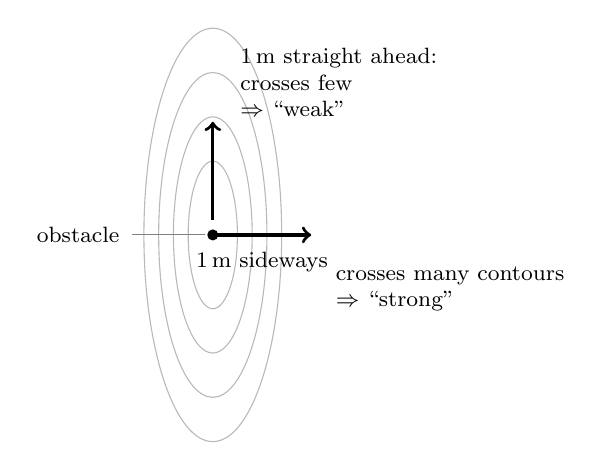
\begin{tikzpicture}[scale=1.25]
  % stretched contours
  \foreach \r in {0.5,0.8,1.1,1.4} {
    \draw[gray!55] (0,0) ellipse ({\r*0.5} and {\r*1.5});
  }
  \fill[black] (0,0) circle (1.6pt);
  \node[font=\footnotesize,anchor=east] at (-0.85,0) {obstacle};
  \draw[gray,-] (-0.82,0) -- (-0.08,0);

  % sideways walk
  \draw[->,very thick] (0,0) -- (1.0,0);
  \node[font=\footnotesize,anchor=north] at (0.5,-0.08) {1\,m sideways};
  \node[font=\footnotesize,anchor=west,align=left] at (1.15,-0.55)
    {crosses many contours\\$\Rightarrow$ ``strong''};

  % forward walk
  \draw[->,very thick] (0,0.15) -- (0,1.15);
  \node[font=\footnotesize,anchor=west,align=left] at (0.18,1.55)
    {1\,m straight ahead:\\crosses few\\$\Rightarrow$ ``weak''};
\end{tikzpicture}
\end{center}

\noindent
Same one metre, same field, wildly different contour counts --- entirely
because of how the contours were drawn.

\section{Where the dip actually comes from}

The factorisation $|\nabla U| = |U'(\rho)|\cdot|\nabla\rho|$ says the force
is a product of two things. Here they are, scanning sideways from the
centreline at $9$\,m ahead:

\begin{center}
\begin{tabular}{rrrrr}
\toprule
$x$ & $\rho$ & $|\nabla\rho|$ & $|U'(\rho)|$ & $|\nabla U|$ (product)\\
\midrule
$0.00$ & $0.6000$ & $0.06667$ & $27.7778$ & $1.8519$\\
$0.10$ & $0.6083$ & $0.17706$ & $27.0270$ & $4.7855$\\
$0.20$ & $0.6325$ & $0.32249$ & $25.0000$ & $8.0623$\\
$0.30$ & $0.6708$ & $0.45117$ & $22.2222$ & $10.0260$\\
$0.44$ & $0.7440$ & $0.59380$ & $18.0636$ & $\mathbf{10.7262}$\\
$0.60$ & $0.8485$ & $0.70868$ & $13.8889$ & $9.8427$\\
$1.00$ & $1.1662$ & $0.85818$ & $7.3529$  & $6.3101$\\
$2.00$ & $2.0881$ & $0.95802$ & $2.2936$  & $2.1973$\\
\bottomrule
\end{tabular}
\end{center}

Read the columns separately and the mystery dissolves:

\begin{itemize}
  \item $|U'(\rho)|$ --- the honest quantity --- falls monotonically,
        $27.8\to2.3$. It never rises. It has no dip and no ridge.
  \item $|\nabla\rho|$ --- the exchange rate --- climbs monotonically,
        $0.067\to0.958$. This is the ruler un-stretching as you leave the
        stretched direction.
  \item Their product is \textbf{not} monotone. It rises to $10.73$ at
        $x\approx0.44$ and falls after. That peak is the ridge, and the low
        value at $x=0$ is the dip.
\end{itemize}

The dip is not a property of the risk. It is what you get when a monotone
decay is multiplied by a monotone climb and the climb wins first.

\section{Why the climb wins first}

One more layer, and this is the part worth internalising. Compare the first
two rows. Moving just $0.10$\,m sideways:

\begin{center}
\begin{tabular}{lcc}
\toprule
 & at $x=0$ & at $x=0.10$\\
\midrule
$\rho$          & $0.6000$  & $0.6083$ \quad($+1.4\%$)\\
$|\nabla\rho|$  & $0.06667$ & $0.17706$ \quad($+166\%$)\\
\bottomrule
\end{tabular}
\end{center}

You have barely moved in risk terms --- $\rho$ changed by one percent --- but
the exchange rate has nearly tripled. That mismatch is the engine of the
dip, and it has a clean cause: \textbf{the two quantities vary on different
lateral scales.} Writing $a=|d_{y}|/t_{y}$ for the on-axis value of $\rho$,
\[
  \rho \text{ changes over a lateral scale } \sim a,
  \qquad
  |\nabla\rho| \text{ changes over a lateral scale } \sim a/t_{y} .
\]
The exchange rate moves $t_{y}$ times faster than the distance does. With
$t_{y}=15$ that is a fifteen-fold head start, so near the axis the climb
always outruns the decay.

This also explains why the dip needs a \emph{threshold} on $q$ rather than
appearing always. The climb has a hard ceiling: $|\nabla\rho|$ can rise from
$1/q$ to $1$ and no further --- a total factor of $q$, and nothing more.
Once it saturates near $1$, the monotone decay of $|U'|$ takes over
unopposed. If $q$ is small there is simply not enough room in the climb to
overturn the decay at all, and no dip ever forms. That is the origin of the
$q>\sqrt3$ condition: it is the point at which the ceiling is high enough to
matter.

\section{What dividing does, then}

Nothing clever. It deletes the second column.

\[
  \underbrace{|\nabla U|}_{\text{non-monotone}}
  \;=\;
  \underbrace{|U'(\rho)|}_{\text{monotone}}
  \times
  \underbrace{|\nabla\rho|}_{\text{the artefact}}
  \qquad\Longrightarrow\qquad
  \frac{|\nabla U|}{|\nabla\rho|}=|U'(\rho)| .
\]

What remains is the column that was always well behaved. Since $|U'(\rho)|$
depends on nothing but $\rho$, and $\rho$ grows as you move away from the
centreline in any direction, the result must decay outward. It cannot dip,
at any elongation, because there is no longer a second factor available to
push it back up.

\section{And the direction is untouched}

Worth saying plainly, because it is what makes this usable. $|\nabla\rho|$ is
a \emph{positive number} at every point. Dividing a vector by a positive
number makes it shorter or longer; it cannot turn it. Every arrow in the
quiver plot points exactly where it pointed before --- only the colours
change.

This is the whole difference between this fix and the metric-weighted
alternative $-G^{-1}\nabla U$, which divides the two components by
\emph{different} numbers and therefore does swing the arrows round, flattening
them onto the radial direction and throwing away the sideways push that makes
the vehicle go around the obstacle rather than merely brake behind it.

\section{The one thing you give up}

An honest closing note. Because $|\nabla\rho|$ is not itself a function of
$\rho$ --- it varies from $1/q$ to $1$ around a single ellipse --- the
rescaled field is no longer the gradient of anything. There is no potential
whose downhill direction it is. For a reactive controller this is usually
fine, but it does mean $U$ can no longer serve as a Lyapunov function, and
any stability argument resting on that has to be rebuilt. The companion note
quantifies the size of this effect.

\end{document}
